\documentclass[nolineno]{ieeeaccess}
\usepackage[T1]{fontenc}
\usepackage{amsmath,amssymb,amsthm,booktabs,array,graphicx}
\usepackage{cite,xurl,etoolbox,float,enumitem,needspace}
\usepackage[hidelinks]{hyperref}
\hypersetup{pdftitle={Innovation-Normalized Conformal Prediction for Autoregressive Episodes: Training and Calibration Costs},pdfauthor={Muhammad Umair Raza, Sohail Ahmed, Ammad Ahmed}}
\floatstyle{ruled}
\newfloat{algorithm}{tbp}{loa}
\floatname{algorithm}{Algorithm}
% Research-draft metadata only; retain the class's typography and page geometry.
\makeatletter
\patchcmd{\@maketitle}{Digital Object Identifier\space\@doi}{}{}{\PackageError{inarcp}{Cannot suppress unassigned DOI}{Check the IEEE Access class version.}}
% Access restores its section command before references; add an explicit anchor.
\patchcmd{\thebibliography}{\addcontentsline{toc}{section}{\refname}}{\phantomsection\addcontentsline{toc}{section}{\refname}}{}{\PackageError{inarcp}{Cannot anchor bibliography}{Check the IEEE Access class version.}}
\def\ps@inarcpdraft{\def\@oddhead{}\def\@evenhead{}%
  \def\@oddfoot{\hfil\footerpagefont\thepage\hfil}%
  \let\@evenfoot\@oddfoot}
\let\ps@firstpage\ps@inarcpdraft
\let\ps@titlepage\ps@inarcpdraft
\let\ps@headings\ps@inarcpdraft
\makeatother
\pagestyle{inarcpdraft}
\raggedbottom
% The distributed Access class aliases the title and abstract dimensions.
% Give the inset abstract its own register so its bullet stays inside the title box.
\newlength{\inarcpabstractwidth}
\setlength{\inarcpabstractwidth}{\dimexpr\titlewidth-10pt\relax}
\let\abstractwidth\inarcpabstractwidth
% Access uses font series n for body text; Courier's regular series is m.
\makeatletter\input{t1pcr.fd}\makeatother
\DeclareFontShape{T1}{pcr}{n}{n}{<->ssub*pcr/m/n}{}
\newtheorem{proposition}{Proposition}
\newtheorem{theorem}{Theorem}
\newcommand{\E}{\mathbb{E}}
\newcommand{\PP}{\mathbb{P}}
\newcommand{\R}{\mathbb{R}}
\newcommand{\Var}{\operatorname{Var}}
\newcommand{\tr}{\operatorname{tr}}
\newcommand{\diag}{\operatorname{diag}}
\newcommand{\clip}{\operatorname{clip}}
\newcommand{\calT}{\mathcal{T}}
\newcommand{\se}{\operatorname{se}}
% Generated from saved data.
\newcommand{\AdaptFour}{0.835}
\newcommand{\StudentFour}{1.004}
\newcommand{\NativeFour}{1.149}
\newcommand{\VariableFour}{1.169}
\newcommand{\FutureFour}{0.5708}
\newcommand{\AdaptTwelve}{0.841}
\newcommand{\StudentTwelve}{0.998}
\newcommand{\NativeTwelve}{0.983}
\newcommand{\VariableTwelve}{1.256}
\newcommand{\FutureTwelve}{0.5223}
\newcommand{\MaxIntegralZ}{1.41}
\newcommand{\CurvatureError}{0.00033}
\newcommand{\MaxJacobiError}{0.293}
\newcommand{\PlanOneGain}{0.67}
\newcommand{\PlanMixGain}{0.56}

\newcommand{\OptInvMin}{0.835}
\newcommand{\OptInvMax}{0.842}
\newcommand{\OptNativeMin}{1.149}
\newcommand{\OptNativeMax}{1.153}

\begin{document}
\history{}
\doi{}
\title{Innovation-Normalized Conformal Prediction for Autoregressive Episodes: Training and Calibration Costs}
\author{\uppercase{Muhammad Umair Raza}\authorrefmark{1},
\uppercase{Sohail Ahmed}\authorrefmark{2}, and
\uppercase{Ammad Ahmed}\authorrefmark{3}}
\address[1]{Department of Avionics Engineering, College of Aeronautical Engineering, National University of Sciences and Technology, Risalpur, Pakistan}
\address[2]{MathWorks, United States}
\address[3]{NDMA, Pakistan}
\corresp{Corresponding author: Muhammad Umair Raza (e-mail: uraza@cae.nust.edu.pk).}
\begin{abstract}
Prediction from short autoregressive histories requires intervals that account for uncertain dynamics and variation in episode amplitude. Normalized conformal calibration can remove amplitude from residual scores, but the effect of amplitude heterogeneity on finite-sample efficiency remains relevant because the predictor is estimated from pooled episodes. We analyze innovation-normalized autoregressive conformal prediction (IN-ARCP) for independent episodes. Under stationary Gaussian AR(1) dynamics, we derive the score distribution at an arbitrary fitted coefficient and combine it with a beta order-statistic law and the distribution of a clipped pooled estimator to characterize expected interval length. A local expansion separates coefficient-estimation, calibration and integer-rank costs; the estimation term depends on the fourth-to-second scale-moment ratio. This expansion yields a discrete training--calibration allocation criterion. Four numerical integrations agree with independent Monte Carlo estimates within \MaxIntegralZ{} standard errors. Across 800 fitted datasets, comparisons with classical, learned and scale-equivariant procedures show near parity with the fitted Student reference under common Gaussian dynamics, while native and nonlinear alternatives are shorter in some settings. At a total budget of 300 episodes, two prespecified allocations reduce mean length by 0.67\% and 0.56\% relative to equal allocation. The analysis provides explicit efficiency costs for a tractable episodic model and identifies the assumptions under which innovation normalization and sample allocation are useful.
\end{abstract}
\begin{keywords}
Autoregressive processes, calibration, conformal prediction, expected interval length, experimental design, scale equivariance.
\end{keywords}
\maketitle

\section{Introduction}
Prediction intervals for a scalar signal must represent uncertainty in the next observation while adapting to the information contained in its recent history. In an episodic setting, a collection of independent short recordings supports training and calibration, whereas temporal dependence is confined to each recording. A central difficulty is that recordings may share standardized dynamics but differ substantially in amplitude. An interval calibrated in absolute response units then reflects the amplitude distribution of the calibration population as well as the uncertainty of the forecast.

Normalized split conformal prediction addresses heterogeneous prediction errors by calibrating residuals relative to a covariate-dependent scale \cite{lei2018}. For autoregressive episodes, an innovation-based history scale is particularly natural: it discounts predictable temporal variation and estimates the scale of the unobserved innovation. Under a Gaussian AR(1) model with a known coefficient, this normalization produces a Student pivot. When the coefficient is estimated, however, the same estimate determines both the prediction center and the history normalization. Its error changes the entire calibration-score distribution.

This interaction matters when the available episode budget is limited. Additional training episodes reduce coefficient uncertainty, whereas additional calibration episodes stabilize the prediction threshold. Moreover, a pooled autoregressive fit weights high-amplitude episodes more heavily, even when amplitude cancels from each normalized calibration score. Scale-invariant scores therefore do not by themselves imply that interval efficiency is insensitive to the distribution of training amplitudes. Quantifying this distinction requires an analysis of fitting and calibration together.

We study that problem for innovation-normalized autoregressive conformal prediction (IN-ARCP). The construction is a specialization of normalized split conformal prediction; the analytical objective is its expected interval length under a specified episodic model. The Gaussian AR(1) setting permits an explicit connection between the fitted residual law, finite calibration ranks and coefficient estimation. It also provides a classical reference against which the cost of conformal calibration can be measured. Departures from this model are examined separately to distinguish coverage robustness from efficiency under correct specification.

Section II develops the relation to prior work, research motivation and contributions. Section III defines the procedure and coverage assumptions. Sections IV and V derive the finite-sample characterization, local efficiency expansion and allocation criterion. Sections VI and VII describe the experiments and results. Section VIII discusses their implications and limitations.

\section{Related Work and Research Motivation}
\subsection{Adaptive conformal intervals and scale normalization}
Lei et al.~\cite{lei2018} establish distribution-free regression prediction and study locally adaptive residual normalization. This framework separates the fitted prediction rule from the calibration rank that controls marginal coverage. Dewolf et al.~\cite{dewolf2024} examine conditional validity for heteroskedastic conformal regression, showing the importance of the underlying distributional structure. In the present setting, conditioning on episode scales is possible because a homogeneous score cancels those scales and leaves exchangeable standardized episodes. This argument does not provide coverage at every fixed observed history.

An alternative is to estimate conditional response quantiles. Conformalized quantile regression (CQR) \cite{romano2019} calibrates lower and upper quantile estimates and can accommodate asymmetry as well as varying spread. Skew-adaptive conformal prediction \cite{marques2026} and recent work on tail allocation \cite{wang2026} further emphasize that the choice of interval shape and tail probabilities affects efficiency. IN-ARCP uses a symmetric interval around an autoregressive center. Its Gaussian benchmark consequently addresses a narrower target than efficient prediction for general skewed or multimodal distributions.

\subsection{Expected length and training--calibration allocation}
Dhillon et al.~\cite{dhillon2024} derive finite-sample expressions for expected conformal-set size. Their score-distribution formulation provides the general basis for integrating a random calibration threshold. For autoregressive episodes, using that formulation requires the score law at a possibly misspecified fitted coefficient and an additional average over coefficient estimation.

Le Bars and Humbert~\cite{bars2025} formulate conformal regression in terms of volume minimization and derive finite-sample excess-volume bounds. Their EffOrt and Ad-EffOrt procedures align predictor fitting with interval efficiency. These results motivate comparing innovation normalization with a learned, efficiency-oriented scale, rather than only with unnormalized residual calibration. Yao et al.~\cite{yao2026} obtain nonasymptotic bounds on oracle-length deviation for conformalized quantile and median regression, jointly tracking training size, calibration size and miscoverage. Their bounded-design analysis controls deviations; the present Gaussian analysis instead evaluates expected length and its model-specific leading constants.

Data allocation is itself an established research question. Das et al.~\cite{das2026} develop a general framework for length-optimal training--calibration splits, with regression specializations and data-based allocation. These results establish a broader allocation framework within which the present criterion is an autoregressive specialization. Our allocation criterion uses the explicit coefficients of the autoregressive expansion and retains the discontinuous conformal-rank correction. Its purpose is to translate this model's efficiency analysis into a computable design choice.

\subsection{Temporal dependence and the sampling unit}
Temporal dependence within a predictor's history must be distinguished from dependence between calibration examples. Barber and Pananjady~\cite{barber2026} analyze split conformal prediction for dependent time series, including predictors with memory, and bound coverage loss through a dependence coefficient. Relational conformal prediction \cite{cini2025} addresses correlated time series. These settings require additional treatment of dependence across observations or series. Here, each complete history--response pair is sampled as one episode. Independent standardized episodes permit the usual rank argument despite dependence among coordinates within an episode. The results therefore do not directly cover overlapping windows from a single recording.

\subsection{Research gap and motivation}
The cited literature supplies adaptive scores, general expected-size identities, excess-length bounds and allocation theory. The remaining analytical task considered here is specific: characterize how a fitted autoregressive coefficient simultaneously changes the interval center, the innovation scale and the calibration threshold when episodes have heterogeneous amplitudes. A generic rate or expected-size identity does not by itself evaluate these coupled quantities for the clipped pooled estimator.

Three features motivate an explicit calculation. First, a finite-sample coefficient estimate can reach a clipping boundary, producing probability masses that contribute to mean length. Second, amplitude normalization removes scale from calibration scores but leaves a fourth-moment dependence in the variability of pooled fitting. Third, the integer calibration rank introduces allocation differences that a continuous split proportion omits. Resolving these effects provides an interpretable benchmark for assessing when a simple autoregressive conformal construction is sufficient and when a more flexible model is needed.

\subsection{Contributions}
The contributions are as follows.
\begin{enumerate}[leftmargin=*,itemsep=3pt]
\item \textbf{A coupled finite-sample characterization.} We derive the normalized score law for any fixed fitted coefficient and combine it with finite-rank calibration and a Gaussian quadratic-form representation of the pooled estimator. Equations~\eqref{eq:cdf}--\eqref{eq:fullmean} account explicitly for clipping atoms and fixed episode scales.
\item \textbf{Explicit efficiency costs.} Relative to a known-coefficient equivariant benchmark, Theorem~\ref{thm:expansion} separates fitting, calibration and rank-rounding costs. The fitting coefficient identifies the role of amplitude heterogeneity through $\kappa=\E\sigma^4/(\E\sigma^2)^2$.
\item \textbf{A discrete allocation criterion.} Equation~\eqref{eq:plan} and Algorithm~\ref{alg:split} convert the expansion into an integer search over feasible splits, preserving the calibration-rank correction.
\item \textbf{Numerical and comparative evaluation.} Independent integration and simulation assess the analytical formulas. Paired comparisons with eight specified procedures examine correct specification, amplitude transfer and structural departures, while a fixed-budget experiment measures the benefit and limitations of the allocation criterion.
\end{enumerate}
Table~\ref{tab:literature} summarizes the relationship between these contributions and the principal efficiency analyses.

\begin{table*}[t]
\centering\small
\caption{Analytical relationship to selected conformal-efficiency studies.}
\label{tab:literature}
\renewcommand{\arraystretch}{1.15}
\begin{tabular}{p{.19\textwidth}p{.34\textwidth}p{.38\textwidth}}
\toprule
Study & Established analytical target & Role in the present study \\
\midrule
Dhillon et al.~\cite{dhillon2024} & Finite-sample expected conformal-set size & Evaluate the score law and then integrate over the fitted AR coefficient. \\
Le Bars and Humbert~\cite{bars2025} & Volume minimization and excess-volume bounds & Compare with efficiency-oriented fitting using stated native and invariant implementations. \\
Yao et al.~\cite{yao2026} & Length-deviation bounds in training size, calibration size and miscoverage & Derive explicit Gaussian mean-length costs for a pooled episodic estimator. \\
Das et al.~\cite{das2026} & Length-optimal data splitting and regression specializations & Apply model-specific costs with an explicit integer-rank correction. \\
Present study & Expected length under Gaussian AR(1) episodes & Couple score, calibration and clipped fitting laws; quantify heterogeneity and allocation effects. \\
\bottomrule
\end{tabular}
\end{table*}

\section{Problem Formulation and Prediction Method}
\subsection{Episodic sampling and model assumptions}
Write an episode as $X=(H_1,\ldots,H_m,Y)$, with history $H$ observed before the response $Y$ is predicted. Use $N$ training episodes and $n$ calibration episodes, and independent evaluation episodes. Histories have the same fixed length $m\geq2$.

For the rank guarantee, let $X_i=\sigma_i Z_i$ with $\sigma_i>0$. Conditional on the training data and all calibration/test scales, standardized calibration and test episodes must be exchangeable. Independent common-law standardized episodes independent of their scales are sufficient. Gaussianity is unnecessary for this statement.

Exact distributional calculations impose
\begin{align}
X_1\mid\sigma&\sim N(0,\sigma^2),\nonumber\\
X_{j+1}&=\rho X_j+\epsilon_{j+1},\quad j=1,\ldots,m,\label{eq:model}\\
\epsilon_{j+1}\mid\sigma&\overset{\mathrm{iid}}{\sim}N(0,\sigma^2(1-\rho^2)).\nonumber
\end{align}
The initial state and innovations are independent, and $\rho\in(-1,1)$ is common across episodes. The marginal scale is $\sigma$ and the innovation scale is $\tau=\sigma\sqrt{1-\rho^2}$. Zero mean and stationarity are assumptions, not consequences of centering using the future response.

\subsection{Innovation-normalized conformal construction}
On training data, set $X_{i,m+1}=Y_i$ and estimate
\begin{align}
\widetilde\rho&=
\frac{\sum_{i=1}^{N}\sum_{j=1}^{m}X_{ij}X_{i,j+1}}
{\sum_{i=1}^{N}\sum_{j=1}^{m}X_{ij}^{2}},\nonumber\\
\widehat\rho&=\clip(\widetilde\rho,-a,a),
\label{eq:fit}
\end{align}
with $a=0.98$. Training responses can enter the fit because they are observed training data. Calibration and test responses do not enter it. High-amplitude training episodes receive greater weight in this pooled estimate.

For fixed $r\in(-1,1)$, define
\begin{equation}
s_r(h)^2=\frac{(1-r^2)h_1^2+\sum_{j=2}^{m}(h_j-rh_{j-1})^2}{m}.
\label{eq:scale}
\end{equation}
At $r=\rho$, the $m$ terms before squaring are independent $N(0,\tau^2)$ innovations. Thus $ms_\rho(H)^2/\tau^2\sim\chi_m^2$. The variance estimate is unbiased; its square root is not an unbiased estimator of $\tau$.

Set $p=1-\alpha$, where $0<\alpha<1$, and
\begin{align}
R_i&=\frac{|Y_i-\widehat\rho H_{im}|}{s_{\widehat\rho}(H_i)},\nonumber\\
k&=\lceil(n+1)p\rceil,\qquad \widehat q=R_{(k)}.
\label{eq:cal}
\end{align}
If $k>n$, use $\widehat q=\infty$. The interval is
\begin{equation}
I(h)=[\widehat\rho h_m-\widehat q\,s_{\widehat\rho}(h),
       \widehat\rho h_m+\widehat q\,s_{\widehat\rho}(h)].
\label{eq:interval}
\end{equation}
The scale uses history only. Positive history scale and training denominator are assumed almost surely. Zero histories are rejected in the implementation; an arbitrary additive scale floor would change exact homogeneity. Fitting costs $O(Nm)$, score evaluation $O(nm)$, and prediction $O(m)$ per episode. Algorithm~\ref{alg:inarcp} specifies the end-to-end construction; Figure~\ref{fig:sequence} shows its implementation call sequence.
\begin{algorithm}[t]
\caption{IN-ARCP: fit, calibrate, and predict}
\label{alg:inarcp}
\small
\textbf{Input:} Training episodes $\mathcal T=\{(H_i,Y_i)\}_{i=1}^N$; separate calibration episodes $\mathcal C=\{(H_i^c,Y_i^c)\}_{i=1}^n$; test history $h_*$; miscoverage $\alpha$; clipping limit $a$ (default $0.98$).\\
\textbf{Require:} $m\geq2$, $N,n\geq1$, $0<\alpha,a<1$; finite, correctly shaped arrays; positive training denominator; nonzero calibration and test histories. The caller enforces the episode-sampling assumptions.\\
\textbf{Output:} Fitted coefficient $r$, threshold $q$, and interval $I(h_*)$.
\begin{enumerate}[label=\arabic*:,leftmargin=1.7em,itemsep=3pt,topsep=5pt]
\item Set $X_i=(H_{i1},\ldots,H_{im},Y_i)$ for training only.
\item Compute $D\gets\sum_{i=1}^N\sum_{j=1}^m X_{ij}^2$.
\item Compute $r\gets\operatorname{clip}\!\left(\dfrac{\sum_{i=1}^N\sum_{j=1}^m X_{ij}X_{i,j+1}}{D},-a,a\right)$.
\item Discard any previous calibration threshold after this fit.
\item \textbf{For each} calibration episode $i=1,\ldots,n$:\\
\hspace*{.6em}$s_i\gets s_r(H_i^c)$ using \eqref{eq:scale};\\
\hspace*{.6em}$R_i\gets |Y_i^c-rH_{im}^c|/s_i$.
\item Set $k\gets\lceil(n+1)(1-\alpha)\rceil$.
\item \textbf{If} $k>n$, set $q\gets+\infty$;\\
\hspace*{.6em}\textbf{else}, set $q\gets R_{(k)}$ without interpolation.
\item Compute $s_*\gets s_r(h_*)$ using \eqref{eq:scale}.
\item \textbf{If} $q=+\infty$, return $(r,q,\mathbb R)$.
\item Set $\mu_*\gets rh_{*m}$ and $w_*\gets qs_*$.
\item Return $(r,q,[\mu_*-w_*,\mu_*+w_*])$.
\end{enumerate}
\textit{Implementation:} The three phases correspond to \texttt{fit}, \texttt{calibrate} and \texttt{predict\_interval}. Numerically equivalent rescaling is used to avoid overflow. Optional allocation (Algorithm~\ref{alg:split}) precedes the data split.
\end{algorithm}

\begin{figure*}[t]
\centering
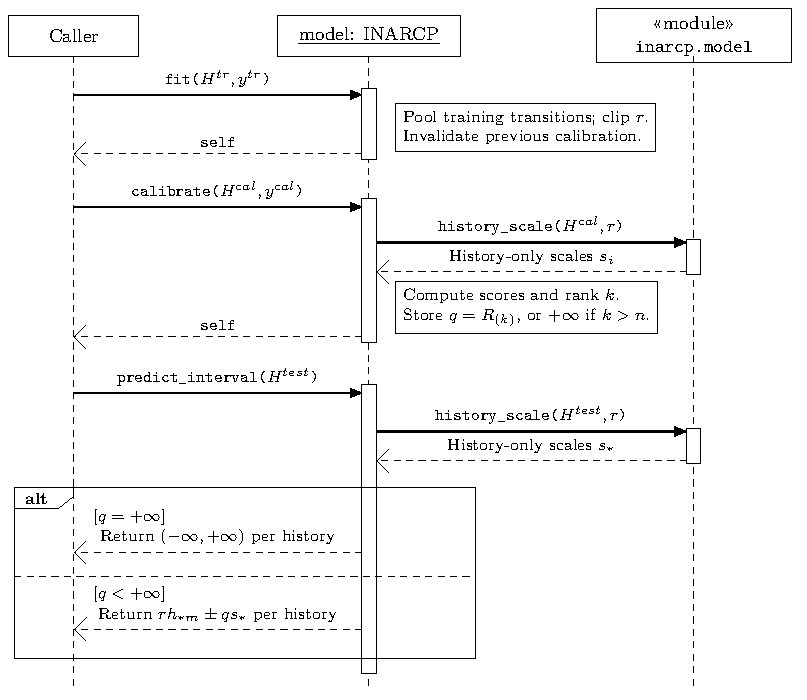
\includegraphics[width=.88\textwidth]{figures/sequence_diagram.pdf}
\caption{UML sequence of the implemented IN-ARCP calls for valid inputs. Solid arrows denote synchronous calls; dashed arrows denote returns; rectangles mark execution. Training uses observed training responses, calibration uses separate observed calibration responses, and prediction receives test histories only. Both prediction branches validate and normalize test histories before returning. The \texttt{alt} guards select one return. Refitting invalidates calibration. Input-validation failures terminate a call and are omitted here. }
\label{fig:sequence}
\end{figure*}

\begin{proposition}[Scale-conditioned coverage]
Under the standardized-episode exchangeability premise,
\begin{equation}
\PP\{Y_*\in I(H_*)\mid\calT,\sigma_1,\ldots,\sigma_n,\sigma_*\}\geq p.
\label{eq:coverage}
\end{equation}
With no score ties and $k\leq n$, coverage is $k/(n+1)$.
\end{proposition}
\begin{proof}
For $c>0$, both the center and $s_r(ch)=cs_r(h)$ are homogeneous. Episode scales therefore cancel from the scores. Conditional on training and scales, the coefficient is fixed and all calibration/test scores are the same function of exchangeable standardized episodes. The corrected rank gives the result.
\end{proof}
This statement integrates over the calibration sample and the standardized test episode. It is not calibration-conditional or history-conditional coverage. Whole-episode scaling satisfies its premise; future-only scaling or changing standardized dynamics generally does not.

\section{Finite-Sample Expected-Length Analysis}
\subsection{Fitted-coefficient score law}
Let $W_r$ be lower bidiagonal with first diagonal entry $\sqrt{1-r^2}$, other diagonal entries one and subdiagonal $-r$. Set $L=W_\rho^{-1}$ and $Q_r=W_r^\top W_r$. Under \eqref{eq:model},
$U=W_\rho H$ and $E=Y-\rho H_m$ are $m+1$ independent $N(0,\tau^2)$ coordinates.

Write $U=RD$, where $D$ is uniform on the sphere in $\R^m$, $R/\tau\sim\chi_m$, and $R,D$ are independent. The variable $V=E/(R/\sqrt m)$ is Student $t_m$ and independent of $D$. Define
\begin{align}
b_r(D)&=\sqrt{D^\top L^\top Q_rLD},\nonumber\\
a_r(D)&=\sqrt m(r-\rho)e_m^\top LD.\label{eq:ab}
\end{align}
The score event is $|V-a_r(D)|\leq q b_r(D)$, so its CDF is
\begin{equation}
G_r(q)=\E_D\!\left[F_m(a_r+qb_r)-F_m(a_r-qb_r)\right],
\label{eq:cdf}
\end{equation}
for $q\geq0$, where $F_m$ is the Student CDF. This law is independent of $\sigma$. At the true coefficient, $G_\rho(q)=2F_m(q)-1$. Replacing $\rho$ by a fitted $r$ does not leave an exact Student pivot.

\subsection{Calibration threshold and expected interval length}
Assume independent common-law standardized calibration episodes and $k\leq n$. Continuity implies
\begin{equation}
\widehat q\overset{d}{=}G_r^{-1}(B),\qquad B\sim\operatorname{Beta}(k,n+1-k).
\label{eq:beta}
\end{equation}
Let
\begin{equation}
A_m=\sqrt{\frac{2}{m}}\frac{\Gamma((m+1)/2)}{\Gamma(m/2)},
\qquad J(r)=\E_D b_r(D).
\end{equation}
Independence of calibration and test episodes yields, for fixed test scale,
\begin{align}
\ell_n(r;\sigma_*)&=2\sigma_*\sqrt{1-\rho^2}\,A_mJ(r)\,M_n(r),\nonumber\\
M_n(r)&=\int_0^1 G_r^{-1}(u)\beta_{k,n+1-k}(u)\,du.
\label{eq:condmean}
\end{align}
This is an exact integral identity, rather than an elementary closed form. For $m\geq2$, the score's polynomial tail of order $m$ gives a finite first moment for every finite calibration rank. If $k>n$, the interval and its mean length are infinite.

Equation \eqref{eq:beta} also explains variation across realized calibration sets: their conditional score coverage $G_r(\widehat q)$ has this beta distribution. Its mean is $k/(n+1)$ and its variance is
\begin{equation}
\frac{k(n+1-k)}{(n+1)^2(n+2)}.
\end{equation}
At $n=19$ and $p=.9$, its central 95\% range is approximately $[.740,.987]$; at $n=1999$ it is $[.886,.913]$. These are sampling ranges over calibration sets, not confidence intervals for a particular application's achieved coverage.

\subsection{Coefficient-estimator distribution and clipping}
Condition on fixed positive training scales $\boldsymbol\sigma=(\sigma_1,\ldots,\sigma_N)$. Let $C$ be a Cholesky factor of the full-episode correlation matrix with entries $\rho^{|j-l|}$. Let $A$ have $1/2$ on the first upper and lower diagonals and zero elsewhere, and $B_0=\diag(1,\ldots,1,0)$. If $\lambda_l(x)$ are eigenvalues of $C^\top(A-xB_0)C$, then
\begin{equation}
\{\widetilde\rho\leq x\}=
\left\{\sum_{i=1}^N\sum_{l=1}^{m+1}\sigma_i^2\lambda_l(x)Z_{il}^2\leq0\right\},
\end{equation}
for independent standard normals $Z_{il}$. Gaussian quadratic-form inversion \cite{imhof1961} gives
\begin{align}
\psi_x(t\mid\boldsymbol\sigma)
 &=\prod_{i,l}(1-2it\sigma_i^2\lambda_l(x))^{-1/2},\nonumber\\
F_N(x\mid\boldsymbol\sigma)
 &=\frac12-\frac1\pi\int_0^\infty\frac{\Im\psi_x(t\mid\boldsymbol\sigma)}{t}\,dt.
\label{eq:trainingcdf}
\end{align}
The continuous complex branch starts at one. Clipping creates atoms $F_N(-a)$ at $-a$ and $1-F_N(a)$ at $a$. Therefore
\begin{align}
\E[|I(H_*)|\mid\boldsymbol\sigma,\sigma_*]
={}&\ell_n(-a;\sigma_*)F_N(-a)\nonumber\\
 &+\int_{(-a,a)}\ell_n(r;\sigma_*)\,dF_N(r)\nonumber\\
 &+\ell_n(a;\sigma_*)[1-F_N(a)].
\label{eq:fullmean}
\end{align}
Omitting the atoms changes this mean. For random independent training scales, an additional expectation over their distribution is required. Independent random test scale with finite mean simply multiplies the unit-scale answer by $\E\sigma_*$.


\section{Asymptotic Efficiency and Sample Allocation}
\subsection{Known-coefficient equivariant benchmark}
Let $c=F_m^{-1}(1-\alpha/2)$. The known-coefficient Student interval $\rho h_m\pm c s_\rho(h)$ has mean length
\begin{equation}
L_* = 2c\sigma_*\sqrt{1-\rho^2}\,A_m.
\label{eq:oracle}
\end{equation}
\begin{proposition}[Oracle within an equivariant class]
Under \eqref{eq:model}, consider measurable intervals with endpoints homogeneous of degree one in the test history. Independent auxiliary information is allowed, with a law fixed as the test scale varies. Among this class, marginal coverage at least $p$ implies expected length at least $L_*$.
\end{proposition}
\begin{proof}
Subtract $\rho H_m$ and divide the endpoints by $R/\sqrt m$. Homogeneity makes the resulting endpoints depend only on $D$ and the auxiliary information. Their nonnegative separation is $L_0$, assigning zero length to empty intervals. The Student pivot is independent of these quantities. For fixed $L_0$, its symmetry and strict unimodality maximize interval probability at centered endpoints. Thus coverage is at most $\E g(L_0)$, where $g(l)=2F_m(l/2)-1$ is increasing and concave. Jensen's inequality implies $p\leq g(\E L_0)$ and hence $\E L_0\geq2c$. Independence of $R$ and $L_0$ gives $\E|I|=\E(R/\sqrt m)\E L_0\geq L_*$. Centered constant normalized width attains equality.
\end{proof}
This is a known-parameter oracle in a restricted class, consistent with classical invariant prediction and relative-efficiency analysis \cite{takada1995,kabaila2007}. It does not assert optimality with an estimated coefficient. A non-equivariant interval can be shorter under one unchanged amplitude population without violating the proposition.

\subsection{Explicit local expansion}
Set $d=1-\rho^2$, $f=f_m(c)$ and
\begin{align}
\kappa&=\frac{\E\sigma^4}{(\E\sigma^2)^2},&
V_\rho&=\frac{d\kappa}{m},\nonumber\\
V_u&=\frac{(m-1)-(m-3+2/m)\rho^2}{m(m+2)d^2},\nonumber\\
K&=\frac{m+1}{2(m+c^2)}\left(c^2V_u+\frac1d\right),\nonumber\\
C_m&=\frac{p(1-p)(m+1)}{8(m+c^2)f^2}.
\label{eq:constants}
\end{align}
\begin{theorem}[Local mean-length expansion]\label{thm:expansion}
Assume independent Gaussian standardized episodes, iid positive training scales independent of shape, and $\E\sigma^{4+\eta}<\infty$ for some $\eta>0$. Fix $m\geq2$, $\alpha\in(0,1)$ and $\rho$ strictly inside the clipping interval. For fixed positive test scale, as $N,n\to\infty$,
\begin{equation}
\begin{aligned}
\frac{\E|I|}{L_*}
={}&1+\frac{KV_\rho}{N}+\frac{C_m}{n+2}
\\ &+\frac{\varepsilon_n}{2cf(n+1)}
+o(N^{-1}+n^{-1}),
\end{aligned}
\label{eq:expansion}
\end{equation}
where $\varepsilon_n=k-(n+1)p\in[0,1)$.
\end{theorem}
Appendix A gives the derivation and expectation control. The three explicit costs arise from coefficient fitting, calibration variation and integer-rank rounding. The result has no finite-sample remainder bound and is not uniform near a unit root, for growing $m$, or as $\alpha$ approaches zero.

Amplitude disappears from the score but remains in learning through $\kappa$. This distinguishes scale-transfer validity from scale-insensitive fitting efficiency. At $\rho=.8$, $\alpha=.1$, $\kappa=1.5$ and $N=1000$, the leading fitting terms are about $0.0227\%$ and $0.0068\%$ for $m=4$ and 12. At $n=1999$, calibration terms are about $0.104\%$ and $0.067\%$. These small costs explain why the Gaussian Student and conformal intervals can be close; they do not explain a much larger gap between differently specified learned methods.

\subsection{Integer allocation of an episode budget}
For $M=N+n$, write $A=KV_\rho$. Ignoring rounding and lower-order offsets gives the continuous planning proportion
\begin{equation}
\frac{N}{M}\approx
\frac{\sqrt A}{\sqrt A+\sqrt{C_m}}.
\label{eq:continuousplan}
\end{equation}
This follows by differentiating $A/N+C_m/(M-N)$. It shows why allocation is model-specific: a single easily estimated coefficient need not consume most of the budget.

Our implemented rule evaluates every feasible integer split:
\begin{align}
n_{\mathrm{plan}}&\in\arg\min_n\,\Phi_M(n),\nonumber\\
\Phi_M(n)&=\frac{A}{M-n}+\frac{C_m}{n+2}
+\frac{\lceil(n+1)p\rceil-(n+1)p}{2cf(n+1)}.
\label{eq:plan}
\end{align}
Algorithm~\ref{alg:split} specifies the integer search, including the finite-rank check and deterministic tie handling.
\begin{algorithm}[t]
\caption{Prespecified integer split planning}
\label{alg:split}
\small
\textbf{Input:} Total episode budget $M$; fixed planning values $(m,\rho,\kappa,\alpha)$; minimum sizes $N_{\min}$ and $n_{\min}$ (defaults 20 and 19).\\
\textbf{Require:} Positive integer counts, $m\geq2$, $\kappa\geq1$, $0<\alpha<1$, and $\rho$ interior to the fitting clip; the expansion's model and moment assumptions.\\
\textbf{Output:} Candidate $(N_{\rm plan},n_{\rm plan})$, or no feasible split.
\begin{enumerate}[label=\arabic*:,leftmargin=1.7em,itemsep=1pt,topsep=3pt]
\item Set $B\gets+\infty$ and $n_{\rm plan}\gets\varnothing$.
\item \textbf{For} $n=n_{\min},\ldots,M-N_{\min}$ in ascending order:
\item \hspace*{.5em}Set $k\gets\lceil(n+1)(1-\alpha)\rceil$.
\item \hspace*{.5em}\textbf{If} $k>n$, continue to the next $n$.
\item \hspace*{.5em}Compute $v\gets\Phi_M(n)$ using \eqref{eq:plan}.
\item \hspace*{.5em}\textbf{If} $v<B$, set $(B,n_{\rm plan})\gets(v,n)$.
\item \textbf{End for.}
\item \textbf{If} $n_{\rm plan}=\varnothing$, report no feasible split and stop.
\item Return $(M-n_{\rm plan},n_{\rm plan})$ and the leading cost $B$.
\end{enumerate}
\textit{Scope:} Strict improvement retains the first minimizer on a tie, matching \texttt{recommend\_split}. Planning values are fixed before calibration or test outcomes are inspected. This minimizes the leading approximation, not the exact finite-sample mean.
\end{algorithm}

Minimum training and calibration sizes are specified beforehand. The rule uses planning values of $\rho,\kappa,m,\alpha$ and never uses calibration/test outcomes to choose a model or split. For unknown planning parameters, an independent pilot or prior engineering assumptions would be needed, with its acquisition cost included. Equation \eqref{eq:plan} minimizes an approximation, not the exact finite-sample mean.

At $M=300$, $m=4$, $\rho=.8$ and $\alpha=.1$, minimum sizes 20 and 19 yield $(N,n)=(61,239)$ for $\kappa=1$, and $(71,229)$ for $\kappa=1.5$. These allocations are fixed before evaluation and compared with alternative prespecified splits.

\section{Experimental Design}
\subsection{Numerical validation of the analytical results}
The study separates numerical verification from empirical comparison. Whitening and precision-determinant identities are checked for five history lengths and five coefficients. At the true coefficient, the finite-calibration mean is independently evaluated by (i) Gauss--Jacobi quadrature of the beta expectation and (ii) adaptive integration. Adjacent $n$ values retain the effect of rank rounding.

Four complete fitted-mean calculations use $m=2$, where directions can be integrated on a circle. Their coefficient CDF uses \eqref{eq:trainingcdf}, with both clipping atoms retained. The coarse calculation uses 64 coefficient bins, 256 midpoint angles and 32 beta nodes; the refined calculation uses 128 bins, 512 angles and 64 beta nodes. Each is compared with 30,000 independent training/calibration repetitions and 32 test episodes per fit. Simulation episodes for these checks are generated by a covariance Cholesky factor, separately from the recurrence generator used in the comparative study.

The calculations span $\rho=.4,.8,.95,-.4$, training counts two or four, equal or unequal fixed training scales, and $n=19$ or 49. This extends verification over clipping and sign changes. It remains a low-history grid; it does not establish uniform numerical accuracy for arbitrary dimension or integrate over every random training-scale law.

\subsection{Data-generating mechanisms and evaluation conditions}
The main experiment uses $N=500$, $n=499$, 1000 evaluation episodes and $\alpha=.1$, with $m\in\{4,12\}$. Every cell has 100 independently fitted repetitions. Four mechanisms give 800 fitted repetitions in total:
\begin{enumerate}
\item stationary Gaussian AR(1), $\rho=.8$;
\item AR(1), $\rho=.8$, with standardized $t_5$ innovations;
\item Gaussian AR(2), coefficients $(.5,.3)$ and innovation variance $0.445714285714$;
\item Gaussian AR(1), with each episode's coefficient independently selected from $\{-.8,.8\}$ with equal probability.
\end{enumerate}
The last three retain common standardized episode distributions across splits but violate the common Gaussian AR(1) efficiency model. Heavy-tailed and AR(2) generators discard 512 initialization steps. Each episode independently receives $\sigma^2=3/G$, $G\sim\operatorname{Gamma}(4,1)$, giving $\E\sigma^2=1$ and $\kappa=1.5$.

Test arms use unchanged amplitude and whole-episode amplitude multiplied by two. These arms rescale the same episodes, so invariant-method coverages are identical up to numerical precision. A Gaussian negative control multiplies only $Y$ by two; it violates the standardized-shape premise.

\subsection{Comparison methods and implementation settings}
All methods share the same training, calibration and evaluation episodes. The primary ablations hold the fitted AR center fixed while using either raw history RMS or an unnormalized, globally calibrated residual. The Gaussian Student reference uses the same fitted coefficient and innovation scale, replacing the calibration quantile by $F_m^{-1}(.95)$. It is not guaranteed to retain coverage under arbitrary innovation distributions.

Linear Ad-EffOrt follows the four-step construction of Le Bars and Humbert~\cite{bars2025}: fit a linear center by smoothed quantile-of-absolute-error optimization, fit a residual quantile function, calibrate residual-minus-radius scores, and add the resulting scalar adjustment to the predicted radius. Its fixed configuration uses 1000 gradient steps proportional to $t^{-.6}$, smoothing $.1$, an intercept and history coordinates, and a 100-tree depth-five residual quantile forest at level $.9$. A vectorized implementation is used for the linear optimizer. The supplement reports its numerical comparison with the authors' implementation and sensitivity to arithmetic and iteration count.

For each invariant adaptation, set $A(H)=\sqrt{m^{-1}\sum_jH_j^2}$; fit and calibrate on $(H/A(H),Y/A(H))$, and rescale predicted test endpoints by $A(H_*)$. This transformation imposes scale equivariance on the learned procedure. Native and invariant Ad-EffOrt are reported separately.

The invariant CQR comparator uses a 100-tree depth-five quantile forest at levels $.05$ and $.95$ and the corrected additive CQR calibration score \cite{romano2019}. The invariant nonlinear comparator uses an RF center with 100 trees, depth eight and minimum leaf size ten, and a residual-scale RF with 100 trees, depth five and minimum leaf size ten, followed by multiplicative calibration. Hyperparameters are fixed across repetitions. Negative adjusted radii or crossed CQR endpoints represent empty sets and contribute zero length and zero coverage, rather than having their endpoints reversed.

\subsection{Performance measures and Monte Carlo uncertainty}
For each fitted repetition, compute coverage and mean length over its evaluation episodes. Monte Carlo standard errors use the variation between fits, following simulation-study principles \cite{morris2019}. For paired mean lengths $L_b,M_b$, let $\widehat R=\overline L/\overline M$. We use
\begin{equation}
\widehat{\se}(\widehat R)=
\frac{\operatorname{sd}(L_b-\widehat R M_b)}
{\sqrt{B}\,\overline M}.
\label{eq:ratiose}
\end{equation}
Displayed 95\% intervals are descriptive Monte Carlo intervals. They are not adjusted for multiple comparisons.

\subsection{Fixed-budget allocation experiment}
The planning study fixes $M=300$, $m=4$, $\rho=.8$, and uses $\kappa=1$ and 1.5. It compares the prespecified candidate in \eqref{eq:plan} against fixed splits, including $150/150$, using 1000 fitted repetitions per setting and 500 test episodes per fit. Within a repetition, splits use the same pool of 300 ordered episodes and the same independent test episodes. The analysis reports all evaluated splits and compares the prespecified recommendation with equal allocation.


\section{Results}
\subsection{Exact means and local calculations}
Table~\ref{tab:integrals} compares the four complete fitted-mean integrations with fresh simulations. The largest discrepancy is \MaxIntegralZ{} Monte Carlo standard errors. The first integral is $6.937226$, reproducing the value reported in the earlier draft through a newly implemented calculation. In the $\rho=.95$ configuration, the upper clipping mass is approximately $.384$; retaining it is consequential.

Whitening, determinant and directional-variance identities agree to floating-point precision on the checked matrix grid. Five deterministic $m=2$ population-curvature checks have maximum relative discrepancy \CurvatureError\%. These checks support the component expressions; they do not turn numerical agreement into a proof.

The finite-calibration integral also reveals a numerical limit. At the most extreme tested finite rank, $m=2,n=9,k=9$, a 512-point Jacobi rule still differs from adaptive integration by \MaxJacobiError\%. The expectation is finite, but its inverse-CDF integrand is singular at one. The default software utility therefore uses adaptive tail integration, and exposes Jacobi quadrature only as an explicit option with refinement guidance.

An additional fitting diagnostic evaluates $N\E(\widehat\rho-\rho)^2$ against $d\kappa/m$. At $N=500$ and $\kappa=1$ or 1.5, the estimates are near the limiting values. At $\kappa=3$, the discrepancies remain substantial: $.2174$ versus $.2700$ for $m=4$, and $.0756$ versus $.0900$ for $m=12$. The expansion is consequently unsuitable as an unchecked finite-sample equality under stronger scale heterogeneity. Figure~\ref{fig:costs} reports this diagnostic alongside calibration costs.

\begin{table*}[t]
\centering\small
\caption{Complete fitted-mean checks, all at $m=2$ and unit test scale. Each Monte Carlo estimate uses 30,000 independent fits. Refinement is the absolute change when all integration grids are increased. Training scales, respectively: $(.7,1.3)$, $(1,1)$, $(.5,1,1.5,2)$, $(.5,1,1.5,2)$.}
\label{tab:integrals}
\begin{tabular}{rrrrrrrr}
\toprule
$\rho$ & $N$ & $n$ & Integral & MC mean & MC SE & Refinement & Discrepancy / SE \\
\midrule
0.40 & 2 & 19 & 6.9372 & 6.9633 & 0.0261 & 0.0039 & 1.00 \\
0.80 & 2 & 49 & 3.8420 & 3.8527 & 0.0076 & 0.0007 & 1.41 \\
0.95 & 4 & 19 & 2.1708 & 2.1648 & 0.0073 & 0.0013 & -0.82 \\
-0.40 & 4 & 49 & 5.6455 & 5.6506 & 0.0112 & 0.0003 & 0.45 \\
\bottomrule
\end{tabular}

\end{table*}

\begin{figure*}[t]
\centering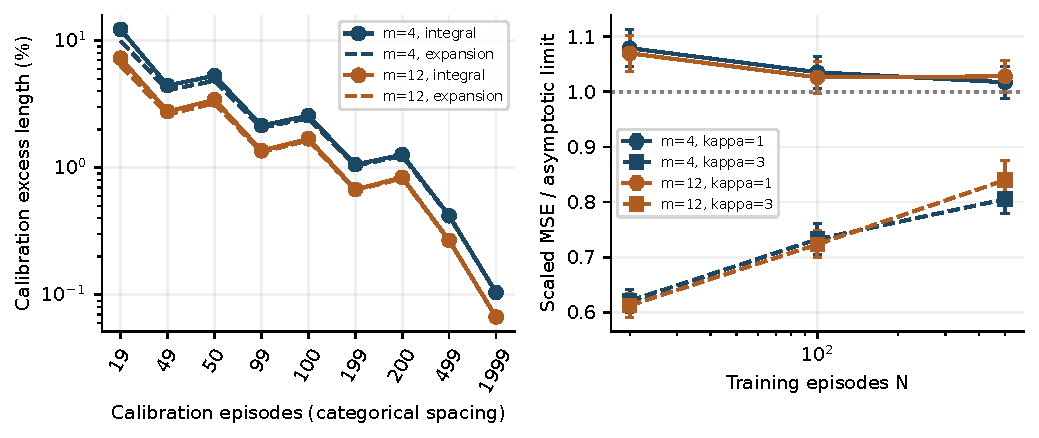
\includegraphics[width=.96\textwidth]{figures/finite_costs.pdf}
\caption{Left: known-coefficient finite-calibration excess length and its leading approximation, retaining integer-rank rounding. Adjacent calibration sizes have categorical spacing. Right: empirical scaled coefficient MSE divided by its asymptotic limit; 10,000 fitted samples per point, with 95\% Monte Carlo intervals. Stronger amplitude heterogeneity causes a material finite-sample discrepancy.}
\label{fig:costs}
\end{figure*}

\subsection{Common Gaussian dynamics}
Table~\ref{tab:common} reports actual coverage and widths for every specified comparator. IN-ARCP's mean-length ratios to the invariant Ad-EffOrt implementation are \AdaptFour{} and \AdaptTwelve{} at $m=4$ and 12. Its ratios to the same-fit Student reference are \StudentFour{} and \StudentTwelve{}, with paired Monte Carlo intervals containing one. The results therefore support efficiency relative to the particular invariant learned comparator while showing near parity with the classical reference.

Against native Ad-EffOrt, the corresponding ratios are \NativeFour{} and \NativeTwelve{}. The $m=4$ result favors the native procedure under unchanged amplitudes. The raw-RMS ablation is longer in both history settings, indicating a benefit from accounting for correlation in the history scale while holding the AR center fixed. Figure~\ref{fig:comparisons} retains all these comparisons.

\begin{table*}[t]
\centering\small
\caption{Fresh common-Gaussian AR(1) comparisons, unchanged amplitude distribution. $N=500,n=499,\alpha=.1$; 100 independent fits per history length. Widths are in the generator's response units. Full per-fit outcomes and Monte Carlo standard errors are supplied.}
\label{tab:common}
\begin{tabular}{lrrrr}
\toprule
Method & Coverage, $m=4$ & Length, $m=4$ & Coverage, $m=12$ & Length, $m=12$ \\
\midrule
IN-ARCP & 0.8985 & 2.318 & 0.8991 & 2.008 \\
AR + raw-RMS & 0.8998 & 2.799 & 0.8986 & 2.253 \\
AR + global & 0.8978 & 1.933 & 0.8972 & 1.923 \\
Student & 0.8988 & 2.309 & 0.9006 & 2.012 \\
Ad-EffOrt native & 0.8975 & 2.017 & 0.8975 & 2.044 \\
Ad-EffOrt invariant & 0.9002 & 2.774 & 0.9001 & 2.387 \\
CQR invariant & 0.8977 & 2.825 & 0.8985 & 2.358 \\
RF invariant & 0.8990 & 2.649 & 0.9001 & 2.318 \\
\bottomrule
\end{tabular}

\end{table*}
\begin{figure*}[t]
\centering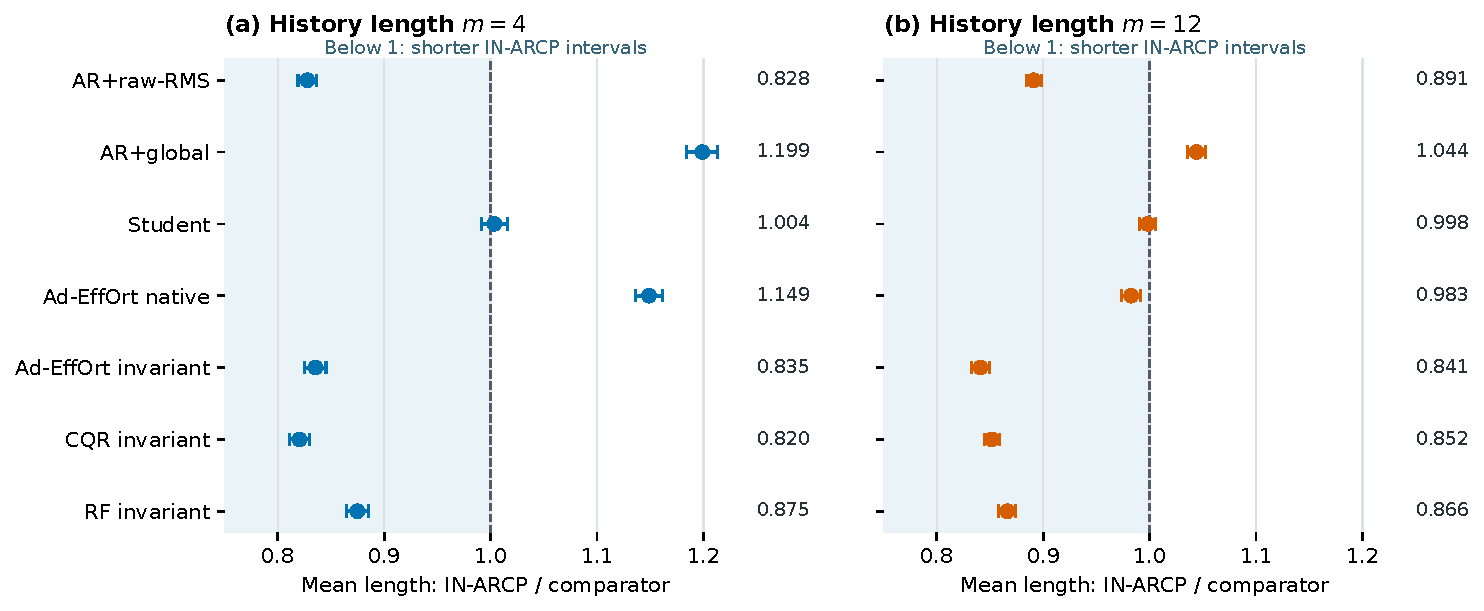
\includegraphics[width=.96\textwidth]{figures/comparisons.pdf}
\caption{Mean-length ratios in the common-Gaussian setting, with paired descriptive 95\% Monte Carlo intervals. Ratios below one favor IN-ARCP in mean length. All methods' coverage estimates are retained in Table~\ref{tab:common}; these comparisons concern fixed implementations and budgets.}
\label{fig:comparisons}
\end{figure*}

Additional implementation checks found numerical path sensitivity in the nonsmooth Ad-EffOrt optimizer. A post-validation Gaussian sensitivity study consequently compares both polynomial arithmetic forms and 1,000/2,000 updates, retaining every configuration. Across these settings, IN-ARCP's ratios to the invariant construction range from \OptInvMin{} to \OptInvMax{}; the native $m=4$ ratios range from \OptNativeMin{} to \OptNativeMax{}. The supplement reports all cells. This check qualifies the comparison as implementation-specific and does not establish exact optimizer equivalence or optimal tuning.

\subsection{Scale transfer and structural changes}
Whole-episode doubling leaves coverage of the invariant constructions unchanged and doubles their widths, as expected from homogeneity. Native Ad-EffOrt and global AR calibration lose coverage in that arm (Table~\ref{tab:shift}). Future-only doubling reduces IN-ARCP coverage to \FutureFour{} and \FutureTwelve{}. This is an expected boundary of the proposition, not a failure under its stated premise.

The structural challenges also produce meaningful losses. For independently varying episode coefficients, IN-ARCP has \VariableFour{} and \VariableTwelve{} times the mean length of the invariant nonlinear RF comparator at similar observed coverage. The direction of this result agrees with the limits of a shared linear center. In the heavy-tailed AR(1) setting, Student coverage is below the target, especially for $m=4$, while conformal calibration remains near the target. CQR, native/adapted Ad-EffOrt and all ablations remain in the complete result tables, including cases where they are shorter.

\begin{table*}[t]
\centering\small
\caption{Gaussian scale-transfer and negative-control coverage. The whole-episode arm rescales the same evaluation episodes. The future-only arm changes standardized shape and is outside the coverage premise.}
\label{tab:shift}
\begin{tabular}{llrrr}
\toprule
$m$ & Method & Unchanged & Whole episode $\times2$ & Future only $\times2$ \\
\midrule
4 & IN-ARCP & 0.8985 & 0.8985 & 0.5708 \\
4 & AR+global & 0.8978 & 0.6203 & 0.5377 \\
4 & Ad-EffOrt native & 0.8975 & 0.7016 & 0.5424 \\
12 & IN-ARCP & 0.8991 & 0.8991 & 0.5223 \\
12 & AR+global & 0.8972 & 0.6175 & 0.5350 \\
12 & Ad-EffOrt native & 0.8975 & 0.7470 & 0.5449 \\
\bottomrule
\end{tabular}

\end{table*}
\begin{table*}[t]
\centering\small
\caption{Structural challenges with unchanged marginal-scale distribution. Ratios are IN-ARCP mean length divided by invariant RF mean length. Whole-episode doubling gives identical coverage and ratios for both invariant methods. The Student column exposes sensitivity of the Gaussian threshold.}
\label{tab:structural}
\begin{tabular}{llrrrrr}
\toprule
Mechanism & $m$ & IN-ARCP cov. & RF cov. & Length ratio & 95\% MC interval & Student cov. \\
\midrule
AR(1), $t_5$ & 4 & 0.8991 & 0.8995 & 0.869 & [0.858, 0.880] & 0.8882 \\
AR(1), $t_5$ & 12 & 0.9029 & 0.9013 & 0.873 & [0.864, 0.881] & 0.8978 \\
AR(2) & 4 & 0.8983 & 0.8994 & 0.927 & [0.918, 0.935] & 0.9014 \\
AR(2) & 12 & 0.9004 & 0.9004 & 0.932 & [0.923, 0.941] & 0.8981 \\
Variable $\rho$ & 4 & 0.9008 & 0.8999 & 1.169 & [1.156, 1.182] & 0.9071 \\
Variable $\rho$ & 12 & 0.9020 & 0.9019 & 1.256 & [1.242, 1.270] & 0.8892 \\
\bottomrule
\end{tabular}

\end{table*}

\subsection{Allocation at a fixed budget}
The prespecified planning candidates reduce mean length relative to the equal $150/150$ split by \PlanOneGain\%{} for $\kappa=1$ and \PlanMixGain\%{} for $\kappa=1.5$ (Table~\ref{tab:planning}). The paired descriptive intervals lie below a ratio of one in these two evaluations.

The candidates lie near a broad group of efficient splits, rather than at a uniquely resolved empirical minimum. Some neighboring splits have slightly smaller sample means. Figure~\ref{fig:planning} displays every evaluated split and the discrepancy between the leading approximation and Monte Carlo means. These results validate a modest planning use of the theory under the tested parameters, not a general finite-sample optimum or a rule estimated from unknown real-world parameters.

\begin{table*}[t]
\centering\small
\caption{Prespecified allocation candidates versus equal allocation, total budget 300. Each ratio uses 1000 paired fitted repetitions. No empirical winner was selected after evaluating the test episodes.}
\label{tab:planning}
\begin{tabular}{rrrrr}
\toprule
$\kappa$ & Training & Calibration & Ratio to $150/150$ & 95\% MC interval \\
\midrule
1.0 & 61 & 239 & 0.9933 & [0.9889, 0.9978] \\
1.5 & 71 & 229 & 0.9944 & [0.9903, 0.9985] \\
\bottomrule
\end{tabular}

\end{table*}
\begin{figure*}[t]
\centering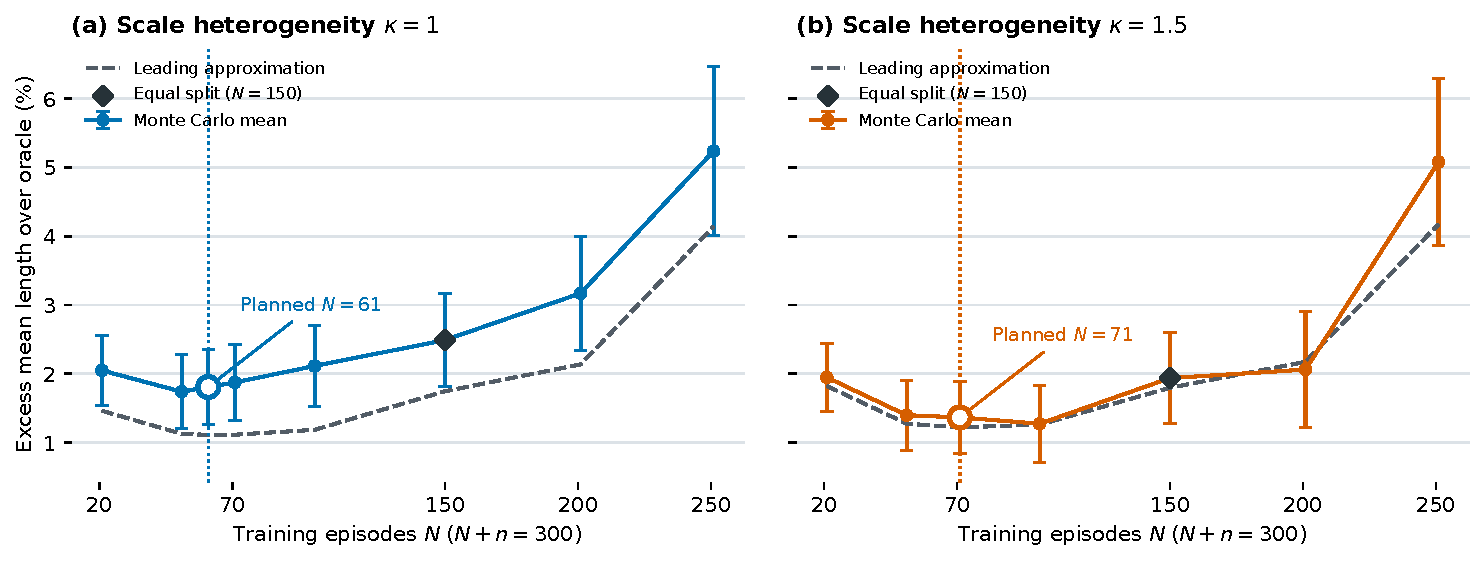
\includegraphics[width=.96\textwidth]{figures/planning.pdf}
\caption{Fixed-budget mean-length excess over the Gaussian equivariant oracle. Bars are descriptive 95\% Monte Carlo intervals for each mean, not paired differences. Dashed curves show the leading approximation; vertical dotted lines mark prespecified integer planning candidates.}
\label{fig:planning}
\end{figure*}


\section{Discussion}
\subsection{Interpretation of the efficiency decomposition}
The analysis connects three distributions: coefficient estimation, the normalized calibration score and the test-history scale. The exact conditional mean and clipped-estimator mixture account for training and calibration together. The expansion exposes a specific mechanism: larger training amplitudes can increase pooled-estimator variability through $\kappa$ even when test amplitude cancels from calibration scores.

The Gaussian Student comparison is central to interpretation. When the model is correct and the coefficient is well estimated, a classical threshold already captures most of the attainable equivariant efficiency. Conformal calibration contributes robustness to the standardized episode distribution at a finite calibration cost. Its value is therefore most visible when distributional assumptions are uncertain, while its Gaussian-model length benefit over that reference is small or absent.

\subsection{Scale transfer and the choice of comparison class}
Imposing whole-episode equivariance changes the comparison class. A native learner can exploit the amplitude distribution of its training population and obtain shorter mean intervals under that same population. An invariant adaptation discards that absolute-amplitude information to make a different transfer property available. The native and adapted comparisons answer distinct questions and must remain labeled.

The restricted oracle does not imply that IN-ARCP is universally shortest. Flexible centers may adapt to episode-dependent dynamics; asymmetric or density-based intervals may be preferable for skewed or multimodal response distributions. The tested forests, quantile models and optimizers are particular implementations with fixed budgets. We do not infer a ranking over the original methods' full range of possible learners and hyperparameters.

\subsection{Limitations}
All experiments are synthetic. The exact equations require zero mean, stationarity, common Gaussian AR(1) dynamics and the specified initialization. The rank guarantee instead requires exchangeable standardized episodes conditional on scales and training. Neither is supplied merely by using disjoint array rows: recording provenance must establish the sampling unit. Non-overlapping windows can still be dependent.

The full numerical integrations cover four $m=2$ configurations. Matrix checks span higher $m$, but broad fitted-mean quadrature in higher dimensions and integration over arbitrary random training scales remain open. The asymptotic expansion has no finite-sample remainder bound, and its approximation can deteriorate with heavy amplitude heterogeneity, few training episodes or coefficients close to clipping. The integer planning rule inherits these restrictions. Its evaluation uses the true synthetic planning parameters; practical estimation of those parameters is not validated here.

The comparison includes 100 fits per cell, so the Monte Carlo precision cannot support arbitrarily small method differences. The intervals displayed are descriptive, with no familywise error claim. Training times depend on the host and implementation and are included only as reproducibility diagnostics.

\subsection{Directions for further evaluation}
A meaningful application must specify the scalar observable, units, next-sample horizon, episode boundaries and acquisition process. Mean removal and other fitted preprocessing must be learned without using future responses. Splits should be grouped by the independent recording or physical unit, and changes in standardized dynamics should be assessed. Baselines should include a simple persistence or affine predictor and a flexible model with the same information.

A next-reading interval alone does not establish detection probability, false-alarm control, interference rejection or latent-state tracking accuracy. Those require a separate observation model and task-specific evaluation. The present work supplies an analytical reference for such a study.

\section{Conclusion}
Innovation normalization separates episode amplitude from conformal calibration, but amplitude heterogeneity continues to affect a pooled autoregressive fit. For Gaussian AR(1) episodes, the derived score law and clipped-estimator mixture characterize the resulting expected interval length. The local expansion makes the fitting, calibration and integer-rank contributions explicit and supports a discrete allocation criterion.

The experiments confirm the numerical characterization in four low-dimensional configurations and show that efficiency depends on model structure and the imposed invariance. IN-ARCP closely matches the fitted Student reference under common Gaussian dynamics, while flexible or native alternatives can be shorter in other settings. The evaluated allocations yield small improvements over an equal split. These findings support the method as an analytically interpretable construction for independent episodes; extensions to unknown planning parameters, richer dynamics and independently sampled real recordings remain necessary for broader use.

\section*{Code and data availability}
Source code, simulation configurations, random seeds, per-repetition outcomes and figure-generation scripts are available at \url{https://github.com/razaumair2203-ux/inarcp}. The experiments use synthetic data generated by the specified models. The supplementary material provides complete results, numerical settings and software versions.

\section*{Acknowledgment}
OpenAI Codex assisted in drafting and editing the abstract, Sections I--IX and appendices; organizing the literature; preparing the algorithms, sequence diagram and figures; and developing the implementation, simulation and verification code.

\appendices
\section{Derivation of the local expansion}
\subsection{Population curvature}
Let $q(r)=G_r^{-1}(p)$ and $h(r)=q(r)J(r)/c$. Put $r=\rho+\delta$ and $A=L^\top Q'_\rho L$. Locally,
\begin{align}
b_r(D)&=1+\delta u(D)+\delta^2v(D)+O(\delta^3),\nonumber\\
a_r(D)&=\delta a_1(D),\qquad
q(r)=c+\delta q_1+\delta^2q_2+O(\delta^3),
\end{align}
with $u(D)=D^\top AD/2$ and $a_1(D)=\sqrt m e_m^\top LD$. Expanding \eqref{eq:cdf} at fixed coverage gives
\begin{align}
q_1&=-c\E u,\nonumber\\
q_2+q_1\E u+c\E v
&=-\frac{f'_m(c)}{2f_m(c)}
   \{c^2\Var(u)+\E a_1^2\}.
\label{eq:curvature}
\end{align}
The left side is the quadratic coefficient in $q(r)J(r)$; its linear coefficient vanishes. Uniform-sphere moments yield
\begin{equation}
\Var(u)=\frac{\tr(A^2)-\tr(A)^2/m}{2m(m+2)},
\quad \E a_1^2=\|e_m^\top L\|^2=d^{-1}.
\end{equation}
The precision matrix $Q_r$ has endpoint diagonal entries one, interior entries $1+r^2$ and off-diagonal entries $-r$. Its determinant is $1-r^2$. Differentiation gives
\begin{equation}
\tr A=-2\rho/d,\qquad
\tr(A^2)=2(m-2)/d+2(1+\rho^2)/d^2.
\end{equation}
These identities give $V_u$ in \eqref{eq:constants}. Since $f'_m(c)/f_m(c)=-(m+1)c/(m+c^2)$,
\begin{equation}
h(\rho+\delta)=1+K\delta^2+O(\delta^3).
\label{eq:h}
\end{equation}

\subsection{Fitting contribution and expectation control}
Write $S_i=\sum_{j=1}^{m}X_{ij}\epsilon_{i,j+1}$ and $D_i=\sum_{j=1}^{m}X_{ij}^2$. Then
\begin{equation}
\widetilde\rho-\rho=\frac{\sum_iS_i}{\sum_iD_i},
\quad \E S_i=0,\quad \E D_i=m\E\sigma^2.
\end{equation}
Cross-transition terms in $\Var(S_i)$ vanish by conditioning on the innovation history. Thus $\Var(S_i)=md\,\E\sigma^4$, and the episode central limit theorem and ratio expansion give
\begin{equation}
\sqrt N(\widehat\rho-\rho)\ \Longrightarrow\ N(0,V_\rho).
\end{equation}
The interior-coefficient assumption makes clipping asymptotically negligible.

The extra scale moment supplies $\E|S_i|^{2+\delta_0}<\infty$ for some $\delta_0>0$. Since $D_i>0$ almost surely with positive finite mean, a lower-tail Chernoff bound controls $\sum_iD_i<N\E D_i/2$ exponentially. On its complement, moment bounds for sums of centered $S_i$ give uniform integrability of $N(\widehat\rho-\rho)^2$; bounded clipping controls the exceptional event. Consequently
\begin{equation}
N\E(\widehat\rho-\rho)^2\to V_\rho,\qquad
\E h(\widehat\rho)=1+\frac{KV_\rho}{N}+o(N^{-1}).
\end{equation}
The same uniform-integrability argument controls contributions outside a fixed neighborhood of $\rho$ and justifies taking expectations in \eqref{eq:h}.

\subsection{Calibration and rank rounding}
At the true coefficient, let $g(u)=F_m^{-1}((1+u)/2)$. Then
\begin{equation}
g'(p)=\frac1{2f},\qquad g''(p)=-\frac{f'_m(c)}{4f^3}.
\end{equation}
For $B$ in \eqref{eq:beta},
\begin{equation}
\E B=p+\frac{\varepsilon_n}{n+1},\qquad
\Var(B)=\frac{p(1-p)}{n+2}+O(n^{-2}).
\end{equation}
A second-order expansion of $\E g(B)/c$ gives the calibration and rounding terms in \eqref{eq:expansion}.

Uniform remainder control uses the compact clipping interval. Eigenvalues of the history quadratic form are bounded away from zero there and the normalized center displacement is bounded. Inverse score quantiles grow at most as a constant times $1+(1-u)^{-1/m}$. Local derivatives are bounded near fixed $p$; beta concentration and the endpoint power control the complement. The fitted-coefficient local terms converge continuously to their values at $\rho$, with expectation errors $o(n^{-1})$. Combining the fitting and calibration expansions gives \eqref{eq:expansion}, without requiring a fixed ratio $N/n$.

\section{Numerical evaluation}
For $m=2$, use midpoint angles $\theta_j=2\pi(j+1/2)/J$ and directions $D_j=(\cos\theta_j,\sin\theta_j)^\top$. Equation \eqref{eq:cdf} is integrated on this grid and inverted by bisection at Gauss--Jacobi beta nodes. The training CDF is independently evaluated by adaptive integration of \eqref{eq:trainingcdf}. A Stieltjes sum on the coefficient grid and its two endpoint masses gives \eqref{eq:fullmean}; every refinement changes all relevant grid sizes and is reported.

For known $\rho$, an alternative calculation avoids inverse-CDF endpoint singularities:
\begin{equation}
\E G_\rho^{-1}(B)=
\int_0^\infty
\{1-I_{G_\rho(x)}(k,n+1-k)\}\,dx,
\end{equation}
where $I_z(a,b)$ is the regularized incomplete beta function. This tail integral is the default in the public utility. A Jacobi option remains available for refinement studies. Finite-rank cases near $k=n$ require care because the inverse score CDF diverges at one even though its expectation is finite.

\bibliographystyle{IEEEtran}
\bibliography{references}
\phantomsection
% Restored from the original manuscript, without introducing new author claims.
\begin{IEEEbiography}[{
\includegraphics[width=1in,height=1.25in,clip,keepaspectratio]{figures/umair_original_portrait.png}}]{Muhammad Umair Raza}
received the B.E. degree in avionics engineering from NUST, Pakistan, in 2008. He completed his M.S. studies in avionics engineering (signal and image processing) at Air University, Islamabad, in 2015; the degree was conferred in 2017. He is with the Department of Avionics Engineering, College of Aeronautical Engineering, NUST, Risalpur, Pakistan. His work includes signal processing and sensing systems.
\end{IEEEbiography}
\begin{IEEEbiographynophoto}{Sohail Ahmed}
received a degree in avionics engineering from the College of Aeronautical Engineering, Pakistan, the M.S. degree in telecommunications engineering from NUST, Pakistan, and the Ph.D. degree from the University of Southampton, UK. He is a Senior Application Engineer with MathWorks, USA. His research includes communications and radar signal processing.
\end{IEEEbiographynophoto}
\begin{IEEEbiographynophoto}{Ammad Ahmed}
studied aeronautical engineering (avionics) at the National University of Sciences and Technology, Pakistan. He is an RF Engineer with NDMA, Pakistan.
\end{IEEEbiographynophoto}

\EOD
\vfill
\end{document}
